\documentclass[11pt]{article} % Font size (can be 10pt, 11pt or 12pt) and paper size (remove a4paper for US letter paper)

\usepackage{amsmath,amssymb,amsthm,gensymb}

\usepackage{geometry}
\usepackage{wrapfig}
\usepackage{hyperref}
\hypersetup{
    colorlinks=true,
    linkcolor=black,
    filecolor=magenta,      
    urlcolor=blue,
}
\usepackage[protrusion=true,expansion=true]{microtype} % Better typography
\usepackage{hyperref}
\usepackage{graphicx} % Required for including pictures
\usepackage{wrapfig} % Allows in-line images
\linespread{1.12}
\usepackage{mathtools}
\usepackage[font=footnotesize,labelfont=bf]{caption}
\usepackage[T1]{fontenc} % Required for accented characters

\makeatletter

\newcommand{\bra}[1]{\left\langle #1 \right|}
\newcommand{\ket}[1]{\left|#1\right\rangle}
\newcommand{\braket}[2]{\left\langle#1 |  #2\right\rangle}
\makeatother

%\addbibresource{bibliography.bib}


\author{Amir Karamlou\footnote{Notes LaTeXed by Megan Yamoah for 6.s089 IAP 2019.}\\\href{mailto:karamlou@mit.edu}{karamlou@mit.edu}}
\title{Introduction to Quantum Computing\\Lecture 3: Classical and Quantum Circuits}
\date{Massachusetts Institute of Technology\\6.s089 IAP 2020}

\begin{document}
\maketitle
\newpage
\tableofcontents
\newpage


\section{Introduction}
With our background from previous lectures, we can now take a look at quantum analogues of classical computing gates. In classical computing, bits can be 0 or 1 and $n$ input bits are mapped to $m$ output bits. We also have traditional logical operations, or gates, such as AND, OR, NOT, NAND, and Fanout (copy) [Table \ref{basic_gates}].

\begin{table}[h!]
    \centering
    AND: 
    \begin{tabular}{c|c c}
        out & a & b\\\hline
        0 & 0 & 0\\
        0 & 1 & 0\\
        0 & 0 & 1\\
        1 & 1 & 1\\
    \end{tabular}\;\;
    OR: 
    \begin{tabular}{c|c c}
        out & a & b\\\hline
        0 & 0 & 0\\
        1 & 1 & 0\\
        1 & 0 & 1\\
        1 & 1 & 1\\
    \end{tabular}\;\;
    NAND: 
    \begin{tabular}{c|c c}
        out & a & b\\\hline
        1 & 0 & 0\\
        1 & 1 & 0\\
        1 & 0 & 1\\
        0 & 1 & 1\\
    \end{tabular}
    \caption{Basic classical gates}
    \label{basic_gates}
\end{table}

The set of {AND, OR, NOT} is a universal set of gates. Namely, all other gates can be created from combinations of elements in the universal set. The NAND gate is also universal (with ancila bits) as is the Toffoli gate, which we will discuss later.

We define a reversible gate as a gate where given an output you can figure out the inputs. The Toffoli gate is reversible while the NAND gate is not. Reversibility relates to Landauer's principle which states that:\\

\noindent\textit{For every bit of information erased, you dissipate energy greater than $k_bT\ln2 \approx 10^{-20} \textrm{J}$.}\\

\noindent Since irreversible gates by definition involve the erasure of information. In quantum systems, since our kets evolve by unitary operations which are reversible, we require all quantum gates to be reversible.

\section{Quantum Gates}
\subsection{Single Qubit Gates}
The common single qubit gates are the Pauli matrices

Pauli x, $\sigma_x$ acts as a NOT gate on our computational basis. $\sigma_z$, the PHASE gate, adds a phase to $\ket{1}$. Lastly, $\sigma_y$ adds a global phase (adds the same phase to both basis states) as well as performs a NOT operation. As such, $\sigma_y$ is a combination of $\sigma_x$ and $\sigma_z$. In fact, the Pauli matrices are related by permutation:
\begin{align}
    \sigma_i\sigma_j = \delta_{ij}\mathbb{I} + \epsilon_{ijk}i\sigma_k
    \label{pauli_permute}
\end{align}
which means that we can get all three Pauli gates from just two of them. In Eq. \ref{pauli_permute}, we use the Levi-Civita symbol $\epsilon_{ijk}$.

The Hadamard gate,
\begin{align}
    H=\frac{1}{\sqrt{2}} =
    \begin{pmatrix}
        1 & 1\\
        1 & -1
    \end{pmatrix}
\end{align}
maps
\begin{align}
    \ket{0} \rightarrow \frac{1}{\sqrt{2}}\left(\ket{0}+\ket{1}\right)\nonumber\\
    \ket{1} \rightarrow \frac{1}{\sqrt{2}}\left(\ket{0}-\ket{1}\right).\nonumber
\end{align}
These new states are again orthogonal. The Hadamard gate actually represents a rotation around the line on the x-z plane that is at a 45\degree angle on the Bloch sphere (Fig \ref{fig:bloch}).
\begin{figure}
    \centering
  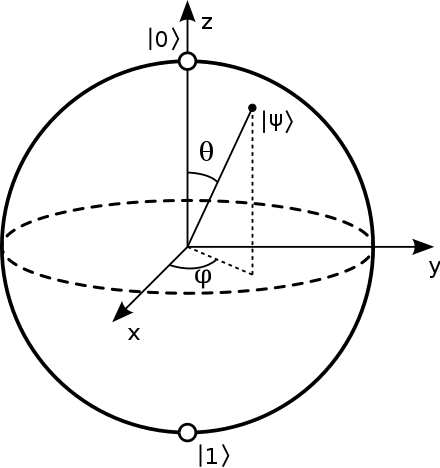
\includegraphics[scale=0.35]{Lecture3Figs/BlochSphere_diag.png}
  \caption{Bloch Sphere}
  \label{fig:bloch}
\end{figure}

\subsection{Two Qubit Gates}
To actually make a useful quantum processor though, we need to have gates for multiple qubits on hand. The most general simple two qubit gate is a controlled unitary which applies a unitary operator on the second qubit based on the state of the first, ``control", qubit. The gate applies the unitary to qubit 2 if the control qubit is in the state $\ket{1}$ and applies the identity otherwise. The 4x4 matrix which represents the action of the two qubit gate in the tensored two qubit space is
\begin{align}
    CU = 
    \begin{pmatrix}
    1 & 0 & 0 & 0\\
    0 & 1 & 0 & 0\\
    0 & 0 & U_{11} & U_{12}\\
    0 & 0 & U_{21} & U_{22}\\
    \end{pmatrix}.
\end{align}

An example of a controlled unitary operator is the CNOT gate which has the unitary equal to $\sigma_x$:
\begin{align}
    CNOT = 
    \begin{pmatrix}
    1 & 0 & 0 & 0\\
    0 & 1 & 0 & 0\\
    0 & 0 & 0 & 1\\
    0 & 0 & 1 & 0\\
    \end{pmatrix}.
\end{align}

The action of CNOT on the state with control bit $\ket{\psi} = \alpha\ket{0}+ \beta\ket{1}$ and target qubit $\ket{\phi} = a\ket{0}+b\ket{1}$ produces entanglement since each part of the control bit's superposition states acts on the target qubit separately.

\section{Universality}
A universal computer can solve any problem. The universal set of gates includes the Clifford gates: \{CNOT, H, S\} plus the T gate where
\begin{align}
    S =
    \begin{pmatrix}
        1 & 0\\
        0 & -i
    \end{pmatrix}
\end{align}
and
\begin{align}
    T =
    \begin{pmatrix}
        1 & 0\\
        0 & e^{-i\pi/4}
    \end{pmatrix}.
\end{align}

\section{No-Cloning Theorem}
In quantum systems, we do not have access to a Fanout, or copy, gate. Namely, any state $\ket{\psi}$ cannot be copied onto another quantum system. Let's begin our proof by supposing we have two identical quantum systems A and B with which we can build a tensored Hilbert space $\mathcal{H}=\mathcal{H}_A\otimes\mathcal{H}_B$ where $\mathcal{H}_A=\mathcal{H}_B$. Now assume we have a unitary operator whose action in $\mathcal{H}$ is to copy the normalized state of system A into the state of system B irrespective of the current state of B. In other words, we define a $U$ in $\mathcal{H}$ such that
\begin{align}
    U(\ket{\psi}_A\ket{e}_B) = e^{i\alpha_{\psi,e}}\ket{\psi}_A\ket{\psi}_B
\end{align}
where we have introduced an arbitrary global phase which has no action on the quantum system but which depends on the initial states $\ket{\psi}$ and $\ket{e}$. Recall that the quantum mechanical state defines a normalized vector in a Hilbert space only up to a phase factor.

We choose two arbitrary initial states of system A: $\ket{\psi}$ and $\ket{\phi}$. Now, we proceed such that
\begin{align}
    \braket{\psi}{\phi}_A\braket{e}{e}_B &= \bra{\psi}_A\bra{e}_B\ket{\phi}_A\ket{e}_B\nonumber\\
    &= \bra{\psi}_A\bra{e}_BU^\dagger U\ket{\phi}_A\ket{e}_B\nonumber\\
    &= e^{i(\alpha_{\phi,e}-\alpha_{\psi,e})}\bra{\psi}_A\bra{\psi}_B\ket{\phi}_A\ket{\phi}_B\nonumber\\
    &= e^{i(\alpha_{\phi,e}-\alpha_{\psi,e})}\left|\braket{\psi}{\phi}\right|^2
\end{align}
which gives us, assuming normalized state $\ket{e}$,
\begin{align}
    \left|\braket{\psi}{\phi}\right| = \left|\braket{\psi}{\phi}\right|^2.
\end{align}

This means that our unitary only for the same or orthogonal states, which contradicts our initial presumption that our unitary works for arbitrary states. So, we no that no such operator exists, proving the no-cloning theorem.




\end{document}